\makeatletter\let\ifGm@compatii\relax\makeatother
\documentclass[9pt,xcolor=pdftex,dvipsnames,table]{beamer}

\usepackage{amsmath}
\usepackage{multirow}
\usepackage{colortbl}
\usepackage{placeins}
\usetheme{Pittsburgh}
%\usetheme{Rochester}
\usecolortheme[RGB={0,75,100}]{structure}
\useinnertheme{circles}

\definecolor{dragonflyblue}{RGB}{0,153,204}
\definecolor{cellyellow}{rgb}{0.988, 0.976, 0.545}
\definecolor{cellorange}{rgb}{0.988, 0.631, 0.357}
\definecolor{cellred}{rgb}{0.890, 0.318, 0.328}
%\definecolor{white}{rgb}{1.0, 1.0, 1.0}
%\setbeamercolor{block title}{fg=white,bg=dragonflyblue}
\setbeamercolor{frametitle}{fg=white}
\setbeamertemplate{navigation symbols}{}

\newcommand\BackgroundPicture[2]{%
    \setbeamertemplate{background}{%
    \parbox[c][\paperheight]{\paperwidth}{%
 \includegraphics[width=#2\paperwidth]{#1}
         \hfill \vfill
      }}}

\newcommand\NoBackground{%
    \setbeamertemplate{background}{}
    }

\newenvironment{narrow}[2]{%
	\begin{list}{}{%
	\setlength{\topsep}{0pt}%
	\setlength{\leftmargin}{#1}%
	\setlength{\rightmargin}{#2}%
	\setlength{\listparindent}{\parindent}%
	\setlength{\itemindent}{\parindent}%
	\setlength{\parsep}{\parskip}}%
	\item[]}{\end{list}}

\usepackage{helvet}
\usepackage{mathptmx}
\usepackage{graphics}
\usepackage[english]{babel}
\usepackage{hhline}
\usepackage{booktabs}
\usepackage{array}
\usepackage{wrapfig}
\usepackage{tikz}

\title[Doing right research]{\textbf{Using the right tools for doing right research}}
\author{Yvan Richard}
\pgfdeclareimage[width=2cm]{damselfly}{/share/dragonfly/templates/logo/damselfly.png}
\institute[Dragonfly Science]
{
Dragonfly Science \\
Level 5, 158 Victoria St, Wellington \\
\medskip
{\emph{yvan@dragonfly.co.nz}}
}

%\texttt{edward@dragonfly.co.nz}

\date[Vic]{26$^{th}$ April 2012}



\begin{document}
\BackgroundPicture{images/banner.png}{1.0}

\begin{frame}
\titlepage
\vspace{-1.5cm}
 \begin{center}
 \resizebox{!}{2cm}{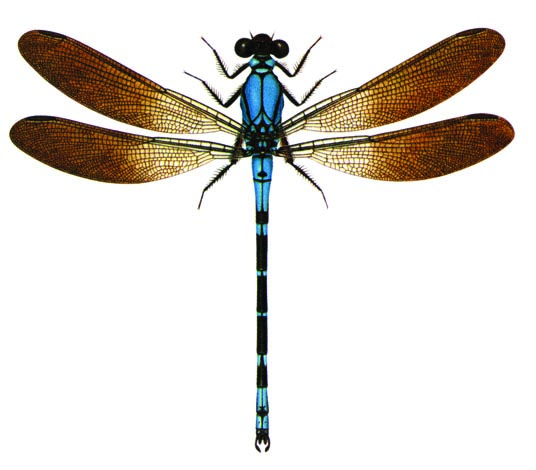
\includegraphics[width=1.2\textwidth]{images/damselfly.png}}
 \end{center}
 \vspace{-2cm}
\end{frame}


\begin{frame}{\textbf{Typical case \#1}}
% \begin{tikzpicture}[remember picture, overlay]
% \node [shift={(-2.5cm, 3.69cm)}] at (current page.south east)
% %\node [shift={(-2.5cm, -2cm)}] at (current page.north east)
% {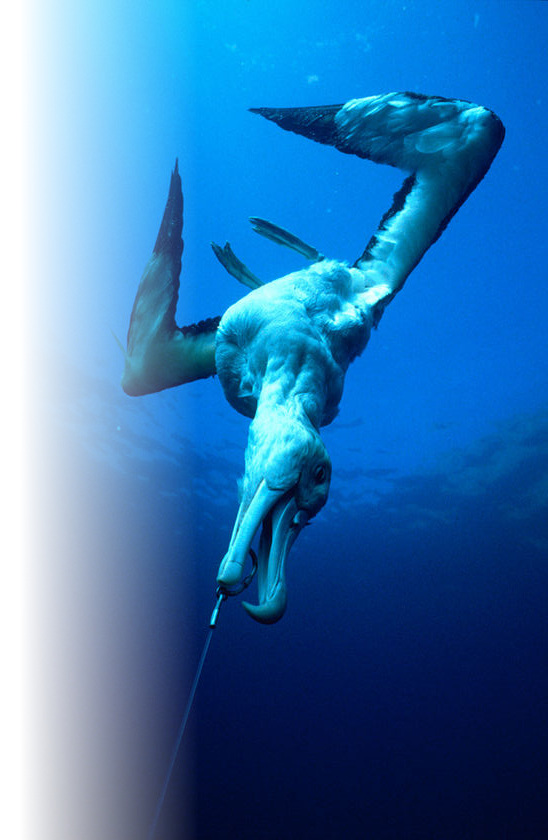
\includegraphics[width=.5\textwidth]{images/grobertson.jpg}};
% \end{tikzpicture}
%\begin{columns}
%\column{0.7\textwidth}
\textbf{New data to be incorporated, or mistake in source data}
\begin{enumerate}
\item Add data to spreadsheet or correct mistake
\item Re-run analyses, involving thousands of clicks
\item Update figures, with a lot of frustration about formatting
\item Update tables, endless copy \& paste operations
\item Update numbers in report -- Have you missed one?
\end{enumerate}
\vspace{0.6cm}
Waste of time, stressful moment, ending up with a vague feeling of
having forgotten to update something...
\vspace{-0.5cm}
\end{frame}

\begin{frame}{\textbf{Typical case \#2}}
\textbf{Accidental deletion or bad direction}
\begin{itemize}
\item You realise at some stage that you deleted some data or some
  text a while ago and that you kept working in a wrong direction.
\item You wish you could go back in time to a previous version of your
  work
\item The deleted part might be lost forever, or at least requires to
  re-do everything since the mistake.
\end{itemize}
\vspace{0.6cm}
Waste of time and frustration! But you learn from your mistake, and
since then, you keep a different version of everything every time you
change something.
\vspace{-0.5cm}
\end{frame}

\begin{frame}{\textbf{Typical case \#3}}
\textbf{Coming back to an old project}
\begin{itemize}
\item The review of a submitted paper comes back and requires you to
  do additional analyses
\item You open your project folder only to discover 20-odd different
  versions of the data
\item Which one did you use?
\item After being fairly confident of the correct one to use, you
  re-do the analyses, and find different results!
\item Eventually, you manage by trial and error to find the same
  results and keep going.
\end{itemize}
\vspace{0.6cm}
Waste of time, ending up unsatisfied and not very confident about the results.
\vspace{-0.5cm}
\end{frame}


\begin{frame}{\textbf{Typical case \#4}}
\textbf{Changing computer}
\begin{itemize}
\item After spending a lot of time perfecting the formatting of your
  thesis, presentation, or article, you realise your document looks
  quite different on another computer
\end{itemize}
\vspace{0.6cm}
Panic and frustration...
\vspace{-0.5cm}
\end{frame}


\begin{frame}{\textbf{Typical case \#5}}
\textbf{Changing institution}
\begin{itemize}
\item After finally getting into grip with a given software, you
  change institution and you realise they use a different
  software. Unfortunately, you cannot get your favourite one because
  the license is too expensive.
\end{itemize}
\vspace{0.6cm}
Waste of time re-learning a new software, never becoming a master at a
given one
\vspace{-0.5cm}
\end{frame}


\begin{frame}{\textbf{Typical case \#6}}
\textbf{Auditing}
\begin{itemize}
\item You work on a sensitive issue, e.g. an endangered species at
  risk of a proposed development project.
\item The ``bad guys'' do not really like your results, preventing
  their project to be approved.
\item In the environmental court, it is agreed that your project gets
  audited, requiring you to show that you get the same results from
  the same data.
\end{itemize}
\vspace{0.6cm}
... Can you?
\vspace{-0.5cm}
\end{frame}



\begin{frame}{\textbf{Typical case \#7}}
\textbf{Teaching}
\begin{itemize}
\item A workmate asks you to show him/her how you do a certain analysis.
\item You sit at a computer with him/her, and start explaining: 
``You go to this menu, and click there, then there, then you go there
and type in that, and then you click on this, etc.''
\item It takes quite a while, as your workmate writes down the whole
  complicated process.
\item He/she gets back to you later, because his/her version of the
  program is slightly different and he/she cannot find a certain item
  in the menus.
\end{itemize}
\vspace{0.6cm}
... (sigh) ...
\vspace{-0.5cm}
\end{frame}


\begin{frame}{\textbf{Let's dream that...}}
\begin{itemize}
\item all these problems could be solved,
\item you could focus on content and process rather than formatting
  and eye-candy,
\item all the tools to solve these problems and do proper research are free,
\item on the way of solving these problems, you acquire great skills
  that would make you find a job very easily.
\end{itemize}
\vspace{0.6cm}
Well, yes, it is possible!
\vspace{-0.5cm}
\end{frame}


\begin{frame}{\textbf{Research}}
Research should:
\begin{itemize}
\item be reproducible
\item be transparent
\item have a functional work flow
\end{itemize}
\vspace{0.6cm}
Sounds trivial, but it is rarely the case!
\vspace{-0.5cm}
\end{frame}


\begin{frame}{\textbf{Scripting power}}
  \begin{itemize}
  \item Everything is written, no lost clicks
  \item Reproducible and transparent
  \item Easily changed
  \item Code is re-usable
  \item Repetitive tasks are done using loops
  \item Generally quicker than clicks and navigating menus
  \item Don't Repeat Yourself (DRY) philosophy
  \end{itemize}
\end{frame}


\begin{frame}{\textbf{Open-source software}}
\begin{itemize}
\item Free!
\item Generally quite portable between operating systems
\item Huge community for support, bug checking and fixing, for new developments
\item Transparent with a non-restrictive license, allowing easy
  communications between programs.
\end{itemize}
\end{frame}


\begin{frame}{\textbf{Main jobs}}
\begin{itemize}
\item Data preparation, exploration, analysis, and plotting
\item Reporting
\item Bibliography
\item Work flow
\item Version control
\item Distribution
\end{itemize}
\end{frame}

\begin{frame}{\textbf{Data preparation, exploration, analysis \\ and plotting}}
\begin{columns}
\column{0.4\textwidth}
\centering

\includegraphics[width=1\textwidth]{images/r-logo.png}
\column{0.6\textwidth}
\begin{itemize}
\item NZ product!
\item Software environment for statistical computing and graphics
\item Programming language, but easy to learn
\item Works on all systems (Windows, Mac, Linux, ...)
\item Increasing popularity, real threat to commercial products
  (e.g. SAS, SPSS)
\item Evolves fast, expandable with thousands of available packages
\end{itemize}
\end{columns}
\end{frame}

\begin{frame}[fragile] % Notice the [fragile] option beside \begin{frame} %
\frametitle{\textbf{R language}}
\begin{columns}
\column{0.5\textwidth}
\begin{example}[]
\begin{verbatim}
## Load data
dat <- read.csv("file-with-data.csv")

## Data manipulation
dat$var3 <- dat$var1 + dat$var2

## Plot
plot(Xvar, Yvar)
\end{verbatim} % Extra carriage return causes problem wit verbatim %
\end{example}
\column{0.48\textwidth}
\vspace{1.5cm}

\includegraphics[width=1\textwidth]{images/corr.png}
\end{columns}
\end{frame}

\begin{frame}[fragile] % Notice the [fragile] option beside \begin{frame} %
\frametitle{\textbf{R language}}
Fitting a linear model
\begin{verbatim}
mod <- lm(dep ~ var1 + var2)
summary(mod)
\end{verbatim}

\scriptsize{
\begin{verbatim}
Call:
lm(formula = indep ~ var1 + var2)

Residuals:
    Min      1Q  Median      3Q     Max 
-7.8060 -1.3795 -0.0133  1.3950  8.2858 

Coefficients:
            Estimate Std. Error t value Pr(>|t|)    
(Intercept)  0.21056    0.23224   0.907   0.3646    
var1         4.95934    0.02074 239.112   <2e-16 ***
var2         0.04883    0.02062   2.368   0.0179 *  
---
Signif. codes:  0 ‘***’ 0.001 ‘**’ 0.01 ‘*’ 0.05 ‘.’ 0.1 ‘ ’ 1 

Residual standard error: 2.083 on 9997 degrees of freedom
Multiple R-squared: 0.8512,	Adjusted R-squared: 0.8511 
F-statistic: 2.859e+04 on 2 and 9997 DF,  p-value: < 2.2e-16
\end{verbatim} 
}
\end{frame}


\begin{frame}{\textbf{R: advanced graphics}}
\centering
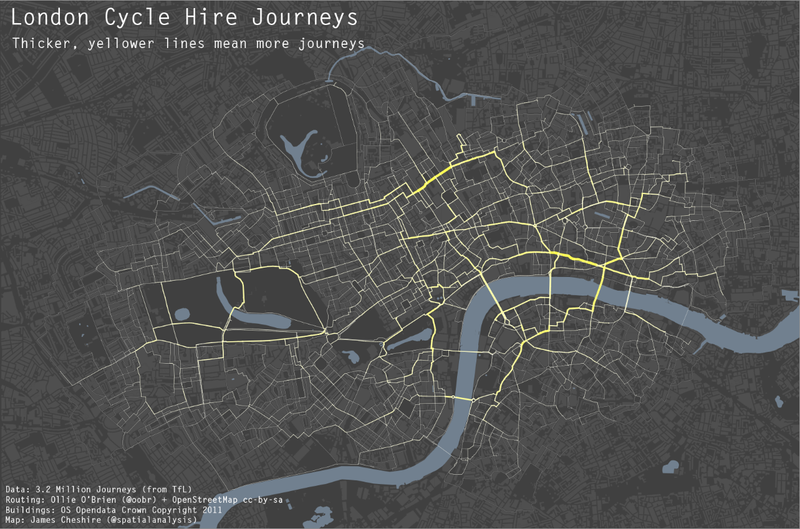
\includegraphics[width=1\textwidth]{images/bike-routes.png}
\vspace{-1cm}
\end{frame}


\begin{frame}{\textbf{Reporting}}
\begin{columns}
\column{0.4\textwidth}
\centering

\includegraphics[width=1\textwidth]{images/LaTeX-logo.png}
\column{0.6\textwidth}
\begin{itemize}
\item Compiled documents, not WYSIWYG
\item Very common
\item Most scientific journals provide their own template
\item Beautiful typesetting
\item Takes care of formatting automatically
\item Maths formulae are easy to write
\item Easy PDF creation with pdflatex
\item Creation of presentations using Beamer (like this one)
\end{itemize}
\end{columns}
\end{frame}


\begin{frame}{\textbf{\LaTeX}}
\centering
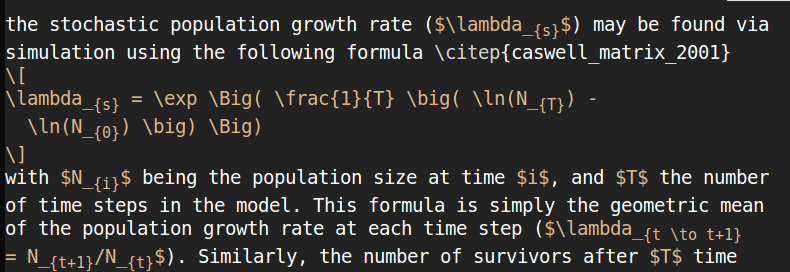
\includegraphics[width=.8\textwidth]{images/latex-ex.png} \\
\vspace{.5cm}
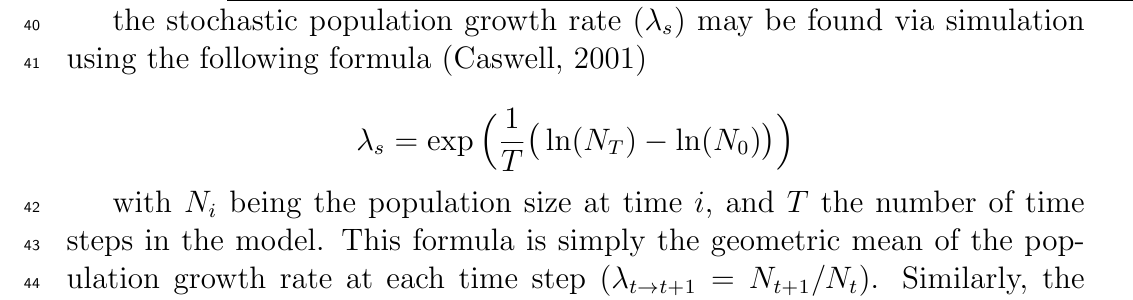
\includegraphics[width=1\textwidth]{images/latex-ex-pdf.png}
\end{frame}


\begin{frame}{\textbf{Calling R into LaTeX using Sweave}}
  \begin{itemize}
  \item Sweave lets data and tables from R to be included in LaTeX documents
  \item Why copying and pasting data manually when you can call them directly?
  \item Enormous time saver
  \item Chances of mistakes are minimal
  \item Initial data can be changed, the changes will be automatically
    reflected in the report 
  \end{itemize}
\end{frame}


\begin{frame}[fragile] % Notice the [fragile] option beside \begin{frame} %
\frametitle{\textbf{Calling R into LaTeX using Sweave}}
\begin{example}[]
\begin{verbatim}
\SweaveOpts{echo=FALSE, results=tex, prefix.string=sweave/fig}

<<load>>=
dat <- read.csv("file-with-data.csv")
minsize <- min(dat$popsize)
maxsize <- max(dat$popsize)
@ 

The population size varied between \Sexpr{minsize} and \Sexpr{maxsize}.
\end{verbatim}
\end{example}
\end{frame}


\begin{frame}[fragile] % Notice the [fragile] option beside \begin{frame} %
\frametitle{\textbf{Bibliography in LaTeX}}
Including references is easy with BibTeX!
References are stored in a text file (e.g.: refs.bib):
\begin{verbatim}
@article{richard_cost_2010,
    title = "Cost distance modelling of landscape connectivity 
             and gap-crossing ability using radio-tracking data",
    volume = "47",
    number = "3",
    journal = "Journal of Applied Ecology",
    author = "Richard, Yvan and Armstrong, Doug P",
    year = "2010",
    pages = "603--610",
    },
\end{verbatim}
Then each reference is called in the LaTeX document by its tag:
\begin{verbatim}
... is a powerful tool to analyse movements \cite{richard_cost_2010}.
\end{verbatim}
\end{frame}


\begin{frame}{\textbf{Bibliography in LaTeX}}
  \begin{itemize}
  \item BibTeX format is very common
  \item References in this format can be downloaded from Google
    Scholar, imported from Zotero, and from journals web site
  \item Templates exist for all journals
  \item No more corrupted EndNote databases...
  \end{itemize}
\end{frame}


\begin{frame}{\textbf{Workflow management}}
\begin{columns}
\column{0.4\textwidth}
\centering
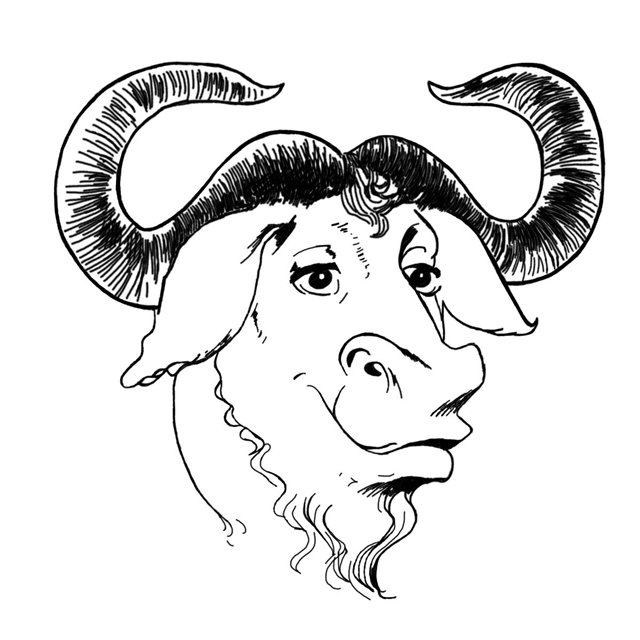
\includegraphics[width=1\textwidth]{images/make-logo.jpg}
\column{0.6\textwidth}
  \begin{itemize}
  \item GNU make
  \item Centralise jobs to be run
  \item Jobs are run in order, and only if necessary
  \item Jobs can be run in parallel in order to use several computer processors
  \item Can be used to document the whole workflow.
  \end{itemize}
\end{columns}
\end{frame}


\begin{frame}[fragile] % Notice the [fragile] option beside \begin{frame} %
\frametitle{\textbf{Workflow management}}
The jobs are written in a text file (makefile):
\small{
\begin{verbatim}
all:  report.pdf

report.pdf:  report.tex datafile.csv refs.bib
    bibtex report 
    pdflatex report

datafile.csv:  analyse.r inputdata.csv
    Rscript analyse.r
\end{verbatim}}
\vspace{0.25cm}
You run the whole process by only typing ``make'' in a terminal, it's
that easy.
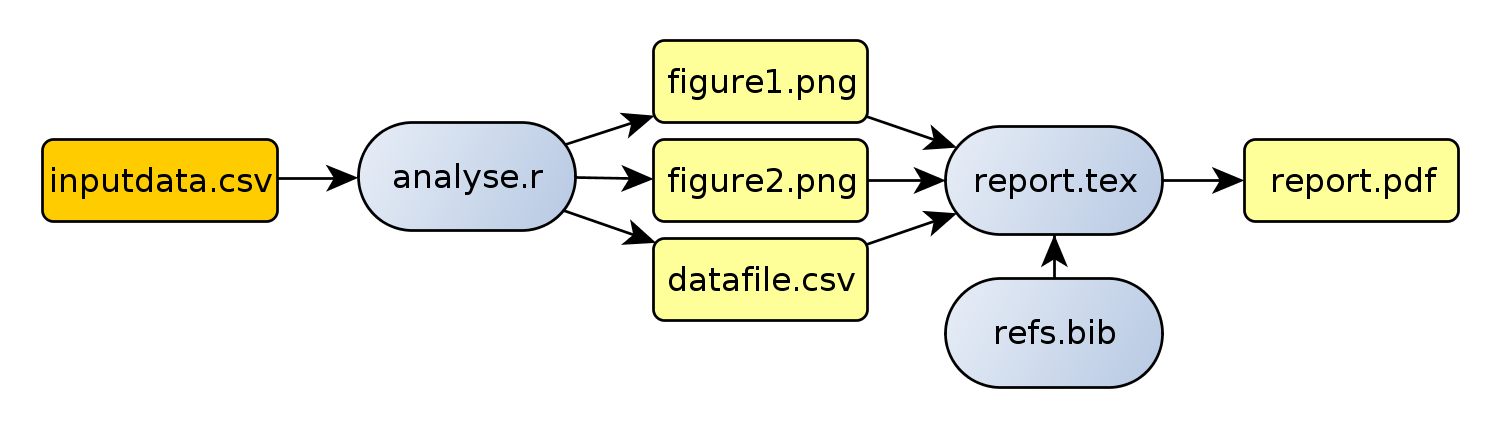
\includegraphics[width=1\textwidth]{images/workflow.png}
\vspace{-1cm}
\end{frame}


\begin{frame}{\textbf{Version control}}
\begin{columns}
\column{0.4\textwidth}
\centering

\includegraphics[width=1\textwidth]{images/git-logo.png}
\column{0.6\textwidth}
\begin{itemize}
\item GIT
\item Saves all gradual changes of files
\item Allows to safely keep only one version of each file 
\item Do not be afraid to delete stuff! You can always come back to previous versions
\item Provides an easy outlook of all modifications
\item Utilities to compare versions
\item Great also for cooperative work
\end{itemize}
\end{columns}
\end{frame}


\begin{frame}[fragile] % Notice the [fragile] option beside \begin{frame} %
\frametitle{\textbf{Workflow management}}
Easy commands: \\
\verb=git status=: to get list of all modified files \\
\verb=git add .=: to inform git to save all modifications \\
\verb=git commit -m "Finished intro of chapter 3"=: to save locally the
current state of modifications, with a comment to describe the changes \\
\verb=git push=: to save the commits to the server
\end{frame}


\begin{frame}{\textbf{Distribution}}
\begin{columns}
\column{0.4\textwidth}
\centering

\includegraphics[width=1\textwidth]{images/github-logo.jpg}
\column{0.6\textwidth}
\begin{itemize}
\item GitHub is a web interface and service to store your git project
\item Makes it easy to access your project from anywhere and to share
  it with others
\item Free for open-source projects
\item Great for issue tracking (to-do list)
\end{itemize}
\end{columns}
\end{frame}



\begin{frame}{\textbf{Conclusions}}
\begin{itemize}
\item Great suite of tools for doing proper research, and it's free!
\item Risk of mistakes minimised
\item Transparent and reproducible
\item Fun! Just like playing Lego
\item Adopting only one of these tools even is a great improvement
  over the traditional bad habits
\item This workflow allows tackling some large projects comfortably
  that would be impossible otherwise
\item These skills will help you all your life and make your life
  easier, and are great to get a job
\item Open research movement; make research more accessible!
\end{itemize}
But...
\begin{itemize}
\item Scary at first; learning curve significant
\end{itemize}
But still worth it 100\%!
\end{frame}


% \begin{frame}{\textbf{Maximum growth rate - $r_{\max}$}}
% \begin{itemize}
% 	\item Life history strategies, allometry. Niel \& Lebreton (2005).
% 	\item Estimated from survival rate ($S$) and age at first reproduction ($A$).
% \end{itemize}
% \vspace{-0.5cm}
% \begin{columns}
% \column{0.3\textwidth}
%     %\begin{footnotesize}
% 	\begin{align*}
% 	\lambda_{max} &= \\
%      & \exp\left[\left(A +{S \over \lambda_{max} - S} \right)^{-1}\right] \\
%     \vspace{1cm} \\
% 	r_{max} &= \lambda_{max}-1 \\ 
% \end{align*}
%     %\end{footnotesize}
% \column{0.75\textwidth}
% 	\begin{block}{}
% 	\centering
% 	\includegraphics[width=1\textwidth]{figures/rmax_survival_age_text_noproxysp_nzmss.png}
% 	\end{block}
% \end{columns}
% \vspace{-1cm}
% \end{frame}


% \begin{frame}{\textbf{Population size - $N_{\min}$}}
% \begin{itemize}
% \item Estimated from survival rate ($S$) and age at first reproduction ($A$).
% \item $N_{\min}$ by taking the lower quartile of the distribution of $N_{\textup{BP}}$.
% \end{itemize}
% \vspace{-0.5cm}
%\begin{columns}
% \column{0.3\textwidth}
% \begin{align*}
% \rho &= S^{1-A} \\ 
% \vspace{1cm} \\
% N_{\textup{tot}} &= \frac{2 N_{\textup{BP}}}{P_\textup{B}} \rho
% \end{align*}
% \column{0.75\textwidth}
% \begin{block}{}
% 	\centering
% 	\includegraphics[width=1\textwidth]{figures/pop_ad_ratio_noproxysp_nzmss.png}
% \end{block}
% \end{columns}
% \vspace{-1cm}
% \end{frame}


% \begin{frame}{\textbf{Potential Biological Removal (PBR)}}
% \begin{itemize}
% \item PBR calculated only from $S$, $A$, $P_\textup{B}$, and $f$.
% \item Estimates of $S$, $A$, and $P_\textup{B}$ from literature, \\groomed to keep best and most recent ones.
% \item 205 final estimates, 65 using proxy species.
% \item $f$ defined according to IUCN red list status,\\ from 0.1 (Critically Endangered) to 0.5 (Least Concern).
% \item Uncertainties from literature or created to match typical values.
% \end{itemize}
% \end{frame}

% %\begin{frame}{\textbf{Approach summary}}
% %\begin{block}{}
% %\centering
% %\includegraphics[width=1\textwidth]{figures/approach_diagram.pdf}
% %\end{block}
% %\vspace{-0.8cm}
% %\end{frame}

% %
% %\BackgroundPicture{figures/captures_pbr.pdf}{0.8}
% %\begin{frame}
% %\begin{columns}
% %\column{0.85\textwidth}
% %\column{0.15\textwidth}
% %\textbf{Captures compared to PBR}
% %\end{columns}
% %\end{frame}
% %
% %\BackgroundPicture{figures/risk_ratios.pdf}{0.8}
% %\begin{frame}
% %\begin{columns}
% %\column{0.85\textwidth}
% %\column{0.15\textwidth}
% %\textbf{Risk ratios}
% %\end{columns}
% %\end{frame}


% %\BackgroundPicture{figures/banner.png}{1.0}
% %\begin{frame}{\textbf{Species potentially at risk}}
% %\begin{itemize}
% %\item Clear risk
% %	\begin{itemize}
% %	\item Parkinson's petrel.
% %	\end{itemize}
% %\item Potentially high
% %	\begin{itemize}
% %	\item NZ king shag, northern royal albatross, Westland petrel, flesh-footed shearwater, Cape petrel, northern giant petrel, grey-headed albatross, Salvin's albatross, Stewart Island shag, yellow-eyed penguin, Chatham albatross, light-mantled albatross, Campbell albatross, Gibson's albatross.
% %	\end{itemize}
% %\item Moderate
% %	\begin{itemize}
% %	\item northern Buller's albatross, Hutton's shearwater, Antipodean albatross, spotted shag, southern Buller's albatross, Fiordland crested penguin, white-chinned petrel, southern royal albatross, grey petrel.
% %	\end{itemize}
% %\item Low
% %	\begin{itemize}
% %	\item Diving petrels, storm petrels, prions, \emph{Pterodroma} petrels, gulls, boobies \& terns.
% %	\end{itemize}
% %\end{itemize}
% %\end{frame}
% \begin{frame}{\textbf{Species at risk}}
% \centering
% \vspace{1cm}
% \includegraphics[width=1\textwidth]{figures/risk_ratios_nzmss.pdf}\\
% %\vspace{1cm} 
% \end{frame}

% \begin{frame}{\textbf{Species at risk - log-normal prior}}
% \centering
% \vspace{1cm}
% \includegraphics[width=1\textwidth]{figures/risk_ratios_priors_nzmss.pdf}\\
% %\vspace{1cm} 
% \end{frame}

% \begin{frame}{\textbf{Side analyses}}
% \begin{tikzpicture}[remember picture, overlay]
% \node [shift={(-3.2cm, 3.90cm)}] at (current page.south east)
% %\node [shift={(-2.5cm, -2cm)}] at (current page.north east)
% {\includegraphics[width=.61\textwidth]{figures/westland_petrel.jpg}};
% \end{tikzpicture}
% \textbf{Sensitivity to uncertainties}
% \begin{itemize}
% \item Inshore fisheries poorly observed
% \item Adult survival rate and number of annual breeding pairs
% \end{itemize}
% \vspace{1cm}
% \textbf{Time variation}
% \begin{itemize}
% \item Captures in trawl fisheries has decreased,\\ following fishing effort and
% the use of mitigation devices.
% \item Possible increase in surface longline fisheries.
% \end{itemize}
% \vspace{-1cm}
% \end{frame}

% %\begin{frame}{\textbf{Black petrel}\\ (\emph{Procellaria parkinsoni})}
% %\begin{columns}
% %\column{0.60\textwidth}
% %\textbf{PBR estimation}
% %\vspace{0.5cm}
% %	\begin{itemize}
% %	\item $N_{\textup{BP}}$ = 1750 breeding pairs (ACAP)
% %	\item $S$ = $90.32\pm2$\% (Bell et al. 2009)
% %	\item $A$ = $6.6\pm0.2$ years (Bell et al. 2009)
% %	\item $f$ = 0.3 (Vulnerable)
% %	\end{itemize}
% %	Therefore,
% %	\begin{itemize}
% %	\item $N_{\min}$ = 6977 birds \\(95\% c.i.: 5314 to 10~210)
% %	\item $r_{\max}$ = 0.092 \\(95\% c.i.: 0.079 to 0.106)
% %	\end{itemize}
% %	And
% %	\begin{itemize}
% %	\item \textbf{PBR = 96 birds (95\% c.i.: 65 to 156)}
% %	\end{itemize}
% %\column{0.40\textwidth}
% %\includegraphics[width=1\textwidth]{figures/black_petrel.jpg}
% %\end{columns}
% %\vspace{-1cm}
% %\end{frame}
% %
% %
% %\begin{frame}{\textbf{Black petrel}\\(\emph{Procellaria parkinsoni})}
% %\begin{columns}
% %\column{0.60\textwidth}
% %	\textbf{Annual captures estimation} \\
% %	\vspace{0.5cm}
% %	29 observed captures.
% %	\begin{columns}
% %	\column{0.5\textwidth}
% %		\includegraphics[width=1\textwidth]{figures/map_PRK_2.png}
% %	\column{0.5\textwidth}
% %		\includegraphics[width=1\textwidth]{figures/map_PRK_4.png}
% %	\end{columns}
% %\column{0.40\textwidth}
% %	\includegraphics[width=1\textwidth]{figures/black_petrel.jpg}
% %\end{columns}
% %\textbf{Total annual captures = 457 birds (95\% c.i.: 322 to 620)} \\
% %$\Rightarrow$ \textbf{Risk ratio = 4.8 (95\% c.i.: 2.6 to 7.9)}
% %\vspace{-1cm}
% %\end{frame}
% %
% %
% %\begin{frame}{\textbf{Black petrel}\\ (\emph{Procellaria parkinsoni})}
% %\begin{columns}
% %\column{0.60\textwidth}
% %	\vspace{-0.5cm}
% %	\begin{small}
% %	\include{tables/prk_captures_fgs}
% %	\end{small}
% %\column{0.40\textwidth}
% %	\includegraphics[width=1\textwidth]{figures/black_petrel.jpg}
% %\end{columns}
% %\textbf{Captures in SNA BLL alone might exceed PBR.}
% %\vspace{-1cm}
% %\end{frame}


% %\begin{frame}{\textbf{Fishery groups}}
% %\begin{itemize}
% %	\item Uncertainty decreases with more observations.
% %	\item Depends on species distribution too.
% %	\item Inshore fisheries poorly observed, or at least in areas of high bird density.
% %		\begin{itemize}
% %		\item Captures of Chatham albatross in small inshore trawl fishery \\
% %= 81 (95\% c.i.: 8 to 368)
% %		\item Captures of Westland petrels in flatfish trawl fishery \\
% %= 68 (95\% c.i.: 8 to 231)
% %		\item Captures of Hutton's shearwater in small bottom longline fishery \\
% %= 254 (95\% c.i.: 22 to 1020)
% %		\end{itemize}
% %	\item Obvious lack of observations in flatfish trawl fishery and in small
% %bottom longline fishery.
% %	\item Large uncertainty in the estimated number of captures due to the lack of observations for almost half the studied species.
% %\end{itemize}
% %\end{frame}


% %\BackgroundPicture{figures/risk_ratios.pdf}{0.8}
% %\begin{frame}
% %\begin{columns}
% %\column{0.85\textwidth}
% %\column{0.15\textwidth}
% %\textbf{Risk ratios}
% %\end{columns}
% %\end{frame}
% %
% %\BackgroundPicture{figures/risk_ratios_priors.pdf}{0.8}
% %\begin{frame}
% %\begin{columns}
% %\column{0.85\textwidth}
% %\column{0.15\textwidth}
% %\textbf{Prior\\ comparison}
% %\end{columns}
% %\end{frame}


% %\BackgroundPicture{figures/banner.png}{1.0}
% %\begin{frame}{\textbf{Hutton's shearwater and small BLL}}
% %\vspace{1cm}
% %\begin{columns}[c]
% %\column{0.5\textwidth}
% %\includegraphics[width=0.7\textwidth]{figures/map_PHU_4.png} \\
% %Species distribution.
% %\column{0.5\textwidth}
% %\includegraphics[width=0.8\textwidth]{figures/map_fishing_effort_fg5_p2003--04_2005--06.pdf} \\
% %Fishing effort and observations. 2003--2006.
% %\end{columns}
% %\end{frame}


% %\begin{frame}{\textbf{Clear interactions}}
% %Some fisheries are well observed.
% %\vspace{0.5cm}
% %\begin{itemize}
% %\item Squid trawl fisheries
% %	\begin{itemize}
% %	\item White-chinned petrel: 196 birds/year (95\% c.i.: 178--215) \\
% %	\item White-capped albatross: 370 birds/year (95\% c.i.: 312--431)
% %	\end{itemize}
% %\item Large BLL fisheries \\
% %	\begin{itemize}
% %	\item White-chinned petrel: 54 birds/year (95\% c.i.: 47--63)
% %	\end{itemize}
% %\item Large SLL fisheries \\
% %	\begin{itemize}
% %	\item Southern Buller's albatross: 72 birds/year (95\% c.i.: 57--89)
% %	\end{itemize}
% %\end{itemize}
% %\end{frame}


% %\begin{frame}{\textbf{Time variation}}
% %%begin{itemize}
% %Some changes in vulnerability and captures over time.
% %	\begin{itemize}
% %	\item Decrease in vulnerability and estimated captures of white-capped
% %    albatrosses in large offshore trawl fishery between 2003--04 to 2005--06
% %    and 2006--07 to 2008--09.\\
% %	Probably due to mitigation devices made compulsory.
% %	\item Increase in vulnerability and in captures in longline fisheries.
% %	\item Decrease in captures in trawl fisheries without obvious change in vulnerability\\
% %	$\Rightarrow$ decrease in fishing effort, no change in fishing practices
% %	\end{itemize}
% %%\end{itemize}
% %\end{frame}
% %
% %
% %\begin{frame}{\textbf{Risk sensitivity to uncertainties}}
% %\begin{itemize}
% %\item Risk uncertainty is driven by the number of breeding pairs, estimated number of annual captures, and adult annual survival rate.
% %\item Risk uncertainty sometimes driven exclusively by one parameter
% %	\begin{itemize}
% %	\item e.g. shags and captures; Buller's albatrosses and survival; prions and number of breeding pairs.
% %	\end{itemize}
% %\end{itemize}
% %\centering
% %\includegraphics[width=0.9\textwidth]{figures/sensitivities.pdf}
% %\vspace{-1.2cm}
% %\end{frame}


% %\begin{frame}{\textbf{Cryptic mortality}}
% %\begin{itemize}
% %\item Not all incidental mortalities recorded.
% %\item Uncertain amount of unobserved mortality from warp strikes, net entanglements, or hook injuries.
% %\item The sensitivity of results to additional mortality was assessed.
% %\item Warp captures $\times 2$ and $\times 10$; hook captures $\times 2$; all captures $\times 2$.
% %\item Risk slightly higher, but qualitatively similar.
% %\end{itemize}
% %\end{frame}
% %
% %
% %\BackgroundPicture{figures/cryptic_mortality.png}{0.55}
% %\begin{frame}
% %\begin{columns}
% %\column{0.85\textwidth}
% %\column{0.15\textwidth}
% %\textbf{Cryptic mortality}
% %\end{columns}
% %\end{frame}




% \BackgroundPicture{figures/banner.png}{1.0}
% \begin{frame}{\textbf{Limitations}}
% \vspace{0.5cm}
% Some intrinsic problems...
% \begin{itemize}
% 	\item Wrong species identification or use of generic codes.
% 	\item Movement in/out the NZEEZ.
% 		\begin{itemize}
% 		\item Captures of birds from outside NZ overestimate risk.
% 			\begin{itemize}
% 			\item e.g. black-browed albatross, Cape petrel, giant petrel?
% 			\end{itemize}
% 		\item Captures of NZ birds outside NZ underestimate risk.
% 			\begin{itemize}
% 			\item e.g. \emph{Procellaria} spp. and albatrosses. 
% 			\end{itemize}
% 		\end{itemize}
% 	\item A few fisheries not included.
% 		\begin{itemize}
% 		\item e.g. recreational, setnet fisheries.
% 		\end{itemize}
% 	\item Other sources of mortality not taken into account underestimate risk.
% 		\begin{itemize}
% 		\item e.g. harvest at colonies, pollution, indirect trophic effects.
% 		\end{itemize}
% 	\item Some birds were captured and released alive, but with unknown fate. They were counted as dead.
% 	\item PBR might often be overestimated.
% 		\begin{itemize}
% 		\item $r_{\max}$, adult ratio.
% 		\end{itemize}
% \end{itemize}
% \end{frame}


% %\begin{frame}{\textbf{Grouping of species}}
% %%\begin{itemize}
% %Some species were grouped because of the lack of observations.
% %	\begin{itemize}
% %	\item e.g. New Zealand king shag, assumed to have the same vulnerability as other shags.
% %		\begin{itemize}
% %		\item No observed captures.
% %		\item Yet, estimated to be potentially at risk.
% %		\item Estimated captures driven by spotted shag.
% %		\end{itemize}
% %	\item Effect unclear.
% %	\end{itemize}
% %%\end{itemize}
% %\end{frame}


% %\begin{frame}{\textbf{Comparison with other studies}}
% %\vspace{0.5cm}
% %Despite limitations, some agreement with other studies.\\
% %\vspace{0.3cm}
% %\begin{itemize}
% %\item Other risk assessments
% %	\begin{itemize}
% %	\item Rowe (2009), expert opinion.
% %		\begin{itemize}
% %		\item Agree: Salvin's albatross, Parkinson's petrel.
% %		\item Disagree: white-chinned petrel, white-capped albatross, sooty shearwater
% %		\end{itemize}
% %	\item Baird \& Gilbert (2010), expert opinion.
% %		\begin{itemize}
% %		\item Agree: Parkinson's petrel, Westland petrel, flesh-footed shearwater
% %		\item Disagree: southern Buller's albatross
% %		\end{itemize}
% %	\item Waugh et al. (2009), similar to our study.
% %		\begin{itemize}
% %		\item Agree: Westland petrel, Chatham albatross, northern royal albatross
% %		\item Disagree: southern Buller's albatross
% %		\end{itemize}
% %	\end{itemize}
% %\vspace{0.3cm}
% %\item Other estimations of captures
% %	\begin{itemize}
% %	\item Abraham et al. (2010).
% %		\begin{itemize}
% %		\item Comparable estimates for sooty shearwater, white-capped albatross, white-chinned petrel.
% %		\item But slightly higher estimates in our study.
% %		\end{itemize}
% %	\end{itemize}
% %\end{itemize}
% %\end{frame}



% %\begin{frame}{\textbf{Comparison of estimated captures}}
% %\centering
% %\vspace{1cm}
% %\includegraphics[width=0.65\textwidth]{figures/estimates_comp.pdf}\\
% %%\vspace{1cm} 
% %\end{frame}


% \begin{frame}{\textbf{Conclusions}}
% \begin{itemize}
% \item Black petrel clearly at risk.
% \item Risk unclear for a few species.
% 	\begin{itemize}
% 	\item Westland petrel, grey-headed albatross, Chatham albatross
% 	\end{itemize}
% \item Some fisheries with obvious lack of observations.
% 	\begin{itemize}
% 	\item Inshore fisheries: especially flatfish trawl, small bottom longline
% 	\end{itemize}
% \item Some flaws potentially important.
% 	\begin{itemize}
% 	\item Movements in/out NZEEZ
% 	\item Lack of seasonality
% 	\item Validation of PBR for seabirds still required
% 	\end{itemize}
% \item Risk assessments can guide management of research and fisheries.
% \end{itemize}
% \end{frame}


% %\begin{frame}{\textbf{Benefits}}
% %\begin{itemize}
% %\item Provide clues on risk of fisheries to seabirds, even with poor data.
% %\item Guide to focus research and management.
% %\item Identify potential actual risk.
% %	\begin{itemize}
% %	\item Fishery, FMA, species
% %	\end{itemize}
% %\item Identify areas of poor knowledge.
% %	\begin{itemize}
% %	\item Observer coverage
% %	\item Demographic parameters
% %	\end{itemize}
% %\item Potentially responsive to changes over time.
% %\end{itemize}
% %\end{frame}

% \begin{frame}{\textbf{Thank you}}
% \begin{tikzpicture}[remember picture, overlay]
% \node [shift={(0cm, 1cm)}] at (current page.south)
% {\includegraphics[width=1.2\textwidth]{figures/flying_birds.jpg}};
% \end{tikzpicture}\textbf{Acknowledgments} \\
% The observers, the Ministry of Fisheries, the members of the Aquatic Environment Working Group, Ben Sharp, Susan Waugh, Elizabeth Bell, Ralph Powlesland, Phil Bradfield, the contributors to the Birdlife Tracking Database, the Agreement on the Conservation of Albatrosses and Petrels.\\ 
% \vspace{0.5cm}
% This research was funded by the Ministry of Fisheries.\\
% \vspace{0.5cm}
% The report can be downloaded from: \\
% http://www.fish.govt.nz/en-nz/Environmental/Seabirds.htm
% \vspace{0.5cm}

% \end{frame}
\end{document}

